\chapter{Planteamiento de la Idea}

Este segundo capítulo se reserva para exponer la idea objeto de esta tésis y la motivación o motivaciones principales que han llevado a su desarrollo, de vital importancia para comprender qué se pretende conseguir con ella y por qué se escogió esta idea y no otra.

\section{Motivación}

La propuesta de la idea para esta tésis proviene del análisis de los factores que hacen distinto el desarrollo y el aprendizaje en este campo, y de cómo estos factores suponen un obstáculo, y en ocasiones incluso un impedimento, a la hora de realizar un proyecto específico.

Por un lado está el ya mencionado factor económico. Si nos paramos a pensar en el motivo por el cual las plataformas existentes se plantean como un servicio por el que hay que pagar caemos en la cuenta de que, aunque haya una parte debida al coste de desarrollo de dicha plataforma y al valor estratégico del producto que cubre una necesidad global en auge, principalmente se debe al consumo de recursos asociado a cualquier proyecto robótico en cualquier ámbito. Trabajar en robótica es sinónimo de disponer de recursos. Es bien sabido que el \textit{hardware} es caro y frágil, que la implementación tanto del sistema físico como de la lógica programada es temporalmente costosa y que incluso con la ausencia de sistemas reales, el coste computacional es enormemente elevado debido a que están involucrados programas exigentes como los simuladores robóticos y también dada la necesidad de un control estricto y veloz de todos los submódulos que componen un proyecto robótico, cada uno de ellos encargado de una tarea que requiere de más y más capacidad para realizar operaciones por unidad temporal. El primer obstáculo encontrado durante el análisis fue precisamente que \textbf{el consumo de recursos genera costes}, y que estos costes son elevados.

Por otro lado, en mi opinión, aprender robótica exige robots. Ya no sólo desde el punto de vista económico sino también desde el logístico, es complicado crear un servicio que disponga de tantos robots como usuarios y que pueda acarrear con los costes derivados de su uso por todo el que lo requiera. Aún pudiendo afrontarlos, construir un sistema que permitiese al usuario, sea estudiante, investigador o simple curioso, evaluar el código de su aplicación sobre un elemento \textit{hardware} remoto y acceder a los resultados en tiempo de ejecución sería una ardua tarea. Por tanto, el análisis realizado destacó que \textbf{desarrollar aplicaciones robóticas requiere disponer de realimentación, visual y paramétrica, en tiempo real}, sólo alcanzable a través de la observación de sistemas electro-mecánicos reales.

Por último, generalmente se desarrolla una gran cantidad de herramientas y plataformas que soportan sistemas específicos, es decir, de funcionalidad acotada. Esto supone un problema para el usuario medio ya que, normalmente, \textbf{carece de \textit{hardware} específico. Sin embargo, sí que tiene acceso a sistemas más básicos}. Esta circunstancia resultó ser la tercera clave extraída del estudio previo.

Con todas ellas y sin perder de vista el objetivo de ``Acercar la robótica a la gente'', se ideó un proyecto que busca sortear esos obstáculos. Quisimos proponer un método que permitiese a la vez minimizar los recursos consumidos por la aplicación robótica y reducir su curva de entrada, que permitiese trabajar indistintamente con entornos simulados y reales y que permitiese al usuario final observar el resultado de su proyecto sobre el robot del que dispone.

\section{Proyecto Planteado}

La \textbf{``Ejecución Mixta''} para proyectos de robótica y visión artificial surge de la conjunción de las ideas anteriormente planteadas, persiguiendo incrementar la accesibilidad de la robótica y su aprendizaje. Se busca elaborar una herramienta que pueda ser conectada de manera modular con cualquier aplicación de carácter robótico y con soporte para cualquier usuario, sean cuales sean sus circunstancias.

Esta idea se planteó con una serie de características intrínsecas que dan forma a los objetivos que se quiere lograr. En tanto que se quiere facilitar el uso de la robótica, deberá existir un Interfaz de Programación o API que abstraiga a los usuarios de todo lo relacionado con la infraestructura de la herramienta y la aplicación, de los mecanismos de comunicación con los sistemas involucrados (tanto robots como sensores y PCs, servidores, \textit{proxys}, etc.) y del control de flujo propio de un sistema complejo, permitiéndole centrarse en su tarea específica de desarrollar con robots. Además, dado que los usuarios potenciales no desean suponer costes sobre los constructores de las aplicaciones que necesitan usar para su trabajo o estudio y que tampoco quieren que se les cobre su utilización (debido en muchos casos a que no se pueden afrontar tasas a largo plazo sin resultados prometedores en plazo corto), la idea que se expone debe estar orientada al cliente, siendo este el que acarree con toda la carga de cómputo posible y asuma el consumo de recursos, que utilizará a su conveniencia según la disponibilidad de la que goce.

Queda de manifiesto que este proyecto busca encajar con aplicaciones docentes y de investigación, actuando más bien como una capa intermedia que hace las funciones de \textit{middleware} entre el robot del usuario y un sistema remoto.

\section{Punto de Partida}

El primer instinto al comenzar el proceso de investigación fue explorar si existía alguna aproximación previa a lo que queríamos conseguir, principalmente para verificar que la solución es posible y no comenzar a caminar por una vía sin salida, y en segunda instancia para partir de algún punto. Encontramos la herramienta \textit{Colaboratory}\footnote{\url{https://colab.research.google.com/notebooks/welcome.ipynb}} de Google, un entorno que permite escribir y ejecutar código, guardar el desarrollo y compartir su análisis por distintos medios, y que tiene funciones que permiten utilizar el \textit{hardware} de aceleración gráfica del equipo que accede a la aplicación para realizar tareas de gran consumo de cómputo haciendo uso de recursos informáticos muy potentes, todo desde el navegador. 

Está construida sobre el proyecto \textit{Jupyter}, que a su vez se ejecuta completamente en la nube, y se utiliza mayoritariamente para el desarrollo  de aplicaciones que tienen que ver con el \textit{Deep Learning}. Así, la gran ventaja que ofrece es que permite a los usuarios descargar su código sobre su propia tarjeta gráfica para acelerar los procesos (Fig. \ref{colab}). Esto se aproxima en cierto modo a nuestros objetivos, aunque en nuestro caso debe extenderse el acceso a todo el \textit{hardware} disponible en la máquina, principalmente. Sin embargo, al encontrar esta herramienta supimos que existía una manera de comunicarse con al menos un elemento \textit{hardware} remoto desde una aplicación de cualquier carácter servida a través de un navegador. Adaptamos y centramos nuestros esfuerzos en esta línea de investigación.

Basándonos en esta estructura existente, continuamos la búsqueda de herramientas para implementar una forma de lograr no sólo la ejecución de código específico accediendo a un único elemento \textit{hardware} concreto de la máquina cliente, sino la ejecución de aplicaciones robóticas completas de cualquier ámbito en cualquier dispositivo \textit{hardware} del que el cliente disponga, incluso si éste está conectado a través de un puerto USB o una red WiFi (ya sea un ordenador, sensores, un robot, etc.) mientras el código se almacena remotamente y se ofrece al usuario a través de la nube, por medio de las tecnologías web. Bajo esta filosofía el código o la aplicación desarrollada por el cliente a través de la web se almacena en un servidor remoto, pero éste sigue teniendo acceso a su análisis y resultados al ejecutarse en sus propios equipos y sistemas robóticos locales, quedando todas las tareas de bajo nivel involucradas en la aplicación robótica ``escondidas'' a nivel de usuario y solventadas por la aplicación que se sirve, como puede ser la comunicación entre servidor y cliente y el acceso a su \textit{hardware}, el diálogo entre el código implementado y robot (simulado o real) y con lo relacionado con el soporte gráfico (UI) y el entorno de trabajo, de modo que se dota al usuario de cierta abstracción de los temas que para él o ella son irrelevantes, permitiéndole centrar sus esfuerzos en idear y desarrollar la lógica que controle al robot y le permita abordar el problema que se propone.

\begin{figure}[!htbp]  \centering\noindent
    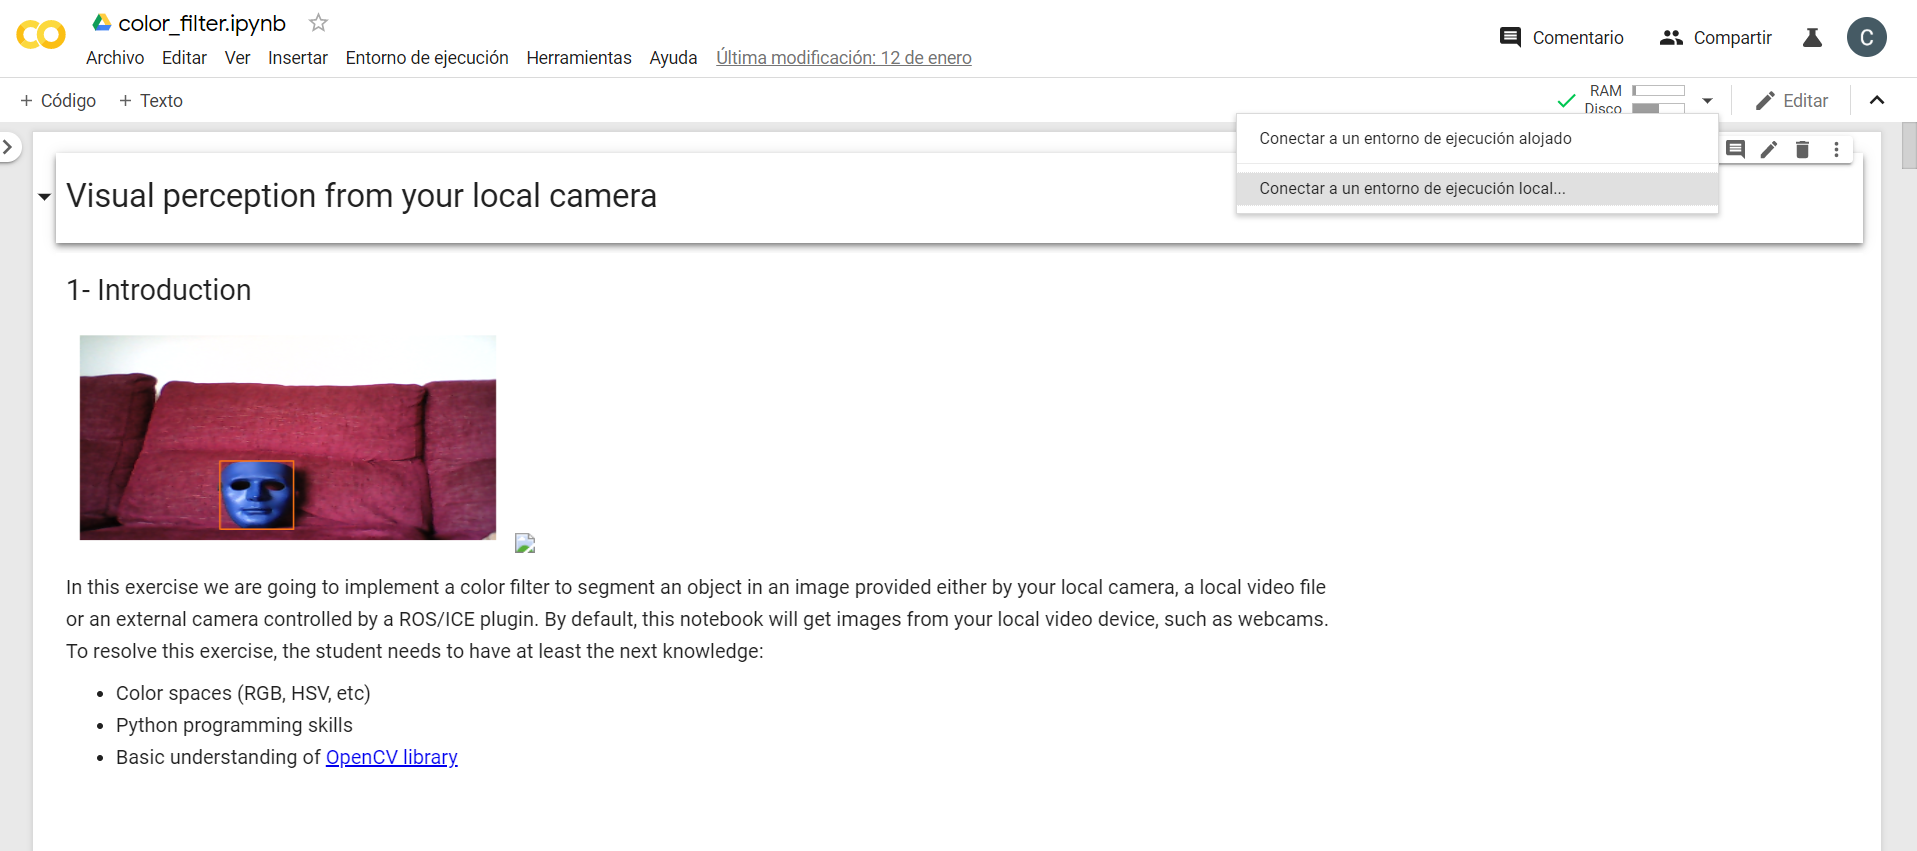
\includegraphics[width=0.99\textwidth,height=7cm]{figures/colab.png}
    \caption{Conexión Local de Colaboratory}
    \label{colab}
\end{figure}
